%! Author = lili
%! Date = 8/12/26


\section{Abgabe 2.1}\label{sec:abgabe-2.1}

\subsection{HA 2.1.1 \abhaken}\label{subsec:ha-2.1.1}
Am Rande des Leinewebermarkts wird Ihnen folgendes Spiel vorgeschlagen.
Es werden zwei faire Würfel geworfen.
Anschließend wird das Maximum und das Minimum der beiden Ergebnisse gebildet.
Der Einsatz des Spiels beträgt zwei Euro, und Sie erhalten die Differenz von Maximum und Minimum ausgezahlt.

\begin{auf}[(a) Geben Sie einen Wahrscheinlichkeitsraum $(\Omega,P)$ an, der es erlaubt, die folgenden Aufgabenteile zu bearbeiten.]
    $\ $
    \begin{figure}[H]
        \centering
        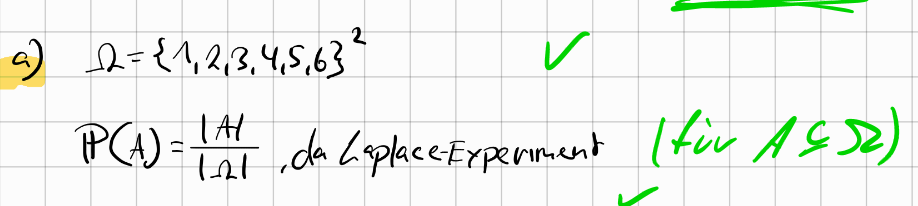
\includegraphics[width=0.8\linewidth]{images/lösungen/wts211a}\label{fig:figure31}
    \end{figure}
\end{auf}

\begin{auf}[(b) Definieren Sie auf dem von Ihnen gewählten Wahrscheinlichkeitsraum $(\Omega,P)$ eine Zufallsvariable $M$, die das Maximum der Ergebnisse der beiden Würfe angibt, und eine Zufallsvariable $N$, die das Minimum der Ergebnisse der beiden Würfe angibt.]
    $\ $
    \begin{figure}[H]
        \centering
        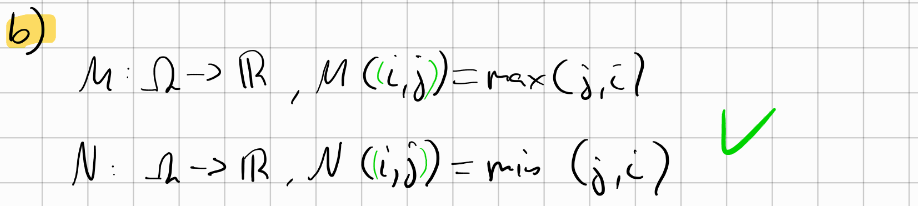
\includegraphics[width=0.8\linewidth]{images/lösungen/wts211b}\label{fig:figure30}
    \end{figure}
\end{auf}

\begin{auf}[(c) Die Zufallsvariable $G:\Omega\to\mathbb R$ bezeichne Ihren Gewinn, sollten Sie eine Runde spielen. Dabei sei $G$ negativ, falls Sie Geld verlieren. Definieren Sie diese Zufallsvariable mit Hilfe der Zufallsvariablen $M$ und $N$, und geben Sie den Bildbereich $G(\Omega)$ an.]
    $\ $
    \begin{figure}[H]
        \centering
        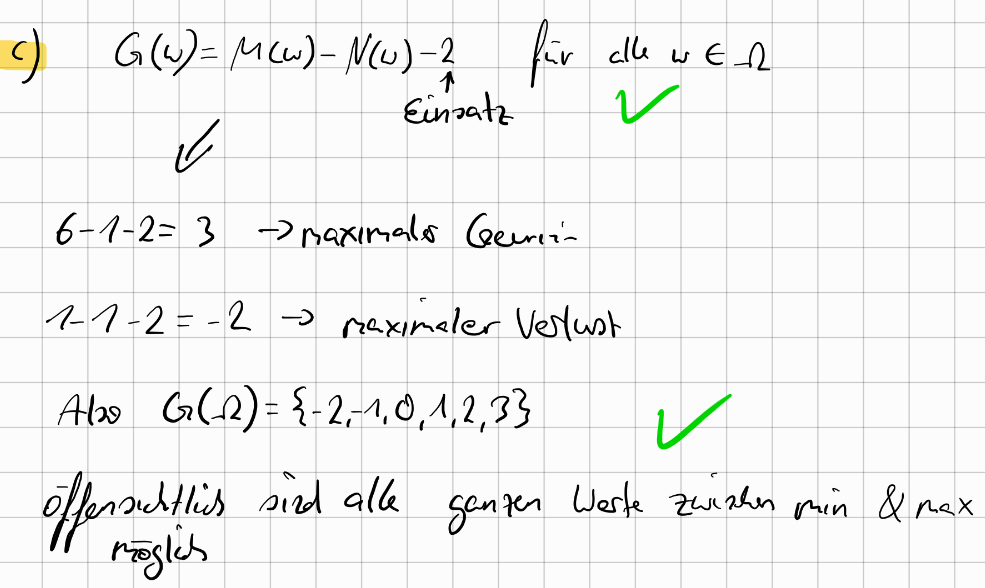
\includegraphics[width=0.8\linewidth]{images/lösungen/wts211c}\label{fig:figure29}
    \end{figure}
\end{auf}

\begin{auf}[(d) Berechnen Sie den erwarteten Gewinn, d.\,h.\ den Erwartungswert von $G$.]
    $\ $
    \begin{figure}[H]
        \centering
        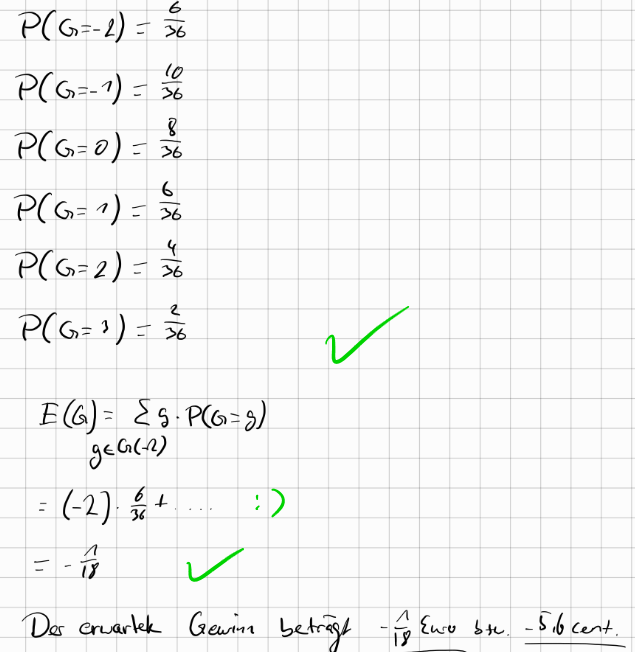
\includegraphics[width=0.8\linewidth]{images/lösungen/wts211d}\label{fig:figure28}
    \end{figure}
\end{auf}

\begin{auf}[(e)  Ist das Spiel fair, das heißt, beträgt der erwartete Gewinn 0 Euro?]
    $\ $
    \begin{figure}[H]
        \centering
        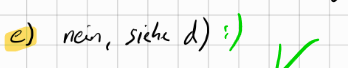
\includegraphics[width=0.8\linewidth]{images/lösungen/wts211e}\label{fig:figure27}
    \end{figure}
\end{auf}



\subsection{HA 2.1.2}\label{subsec:ha-2.1.2}
Die gemeinsame Dichte der Zufallsvariablen $X$ und $Y$ sei gegeben durch
\[
    f(x,y) = \begin{cases}
                 c\,e^{-2(x+y)} & \text{für } 0\le x\le y<\infty, \\
                 0 & \text{sonst}.
    \end{cases}
\]
\begin{auf}[(a) Bestimmen Sie $c$ derart, dass $f$ eine zweidimensionale Dichte ist.]
    NOCH KEINE LÖSUNG % TODO NOCH KEINE LÖSUNG
\end{auf}

\begin{auf}[(b) Berechnen Sie Erwartungswert und Varianz von $X$ und $Y$. Warum existieren diese?]
    NOCH KEINE LÖSUNG % TODO NOCH KEINE LÖSUNG
\end{auf}

\begin{auf}[(c) Berechnen Sie den Erwartungswert von $2X-Y$. Warum existiert dieser?]
    NOCH KEINE LÖSUNG % TODO NOCH KEINE LÖSUNG
\end{auf}

\subsection{HA 2.1.3 (Teils)}\label{subsec:ha-2.1.3}
Anlässlich einer Feier unter $N$ Freundinnen bringt jede Teilnehmerin ein Geschenk mit.
Diese Geschenke werden am Ende der Feier zufällig verteilt, so dass jede der Freundinnen genau ein Geschenk bekommt.

\begin{auf}[(a) Geben Sie einen Wahrscheinlichkeitsraum $(\Omega,P)$ an, der es erlaubt, die folgenden Aufgabenteile zu bearbeiten.]
    NOCH KEINE LÖSUNG % TODO NOCH KEINE LÖSUNG
\end{auf}

\begin{auf}[(b) Wie groß ist die Wahrscheinlichkeit, dass mindestens eine der Freundinnen ihr eigenes Geschenk zurückerhält?]
    NOCH KEINE LÖSUNG % TODO NOCH KEINE LÖSUNG
\end{auf}

\begin{auf}[(c) Bestimmen Sie den Limes dieser Wahrscheinlichkeit für $N\to\infty$.]
    NOCH KEINE LÖSUNG % TODO NOCH KEINE LÖSUNG
\end{auf}

\begin{auf}[(d) Definieren Sie Zufallsvariablen $X_1,\dots,X_N$ auf dem Wahrscheinlichkeitsraum $(\Omega,P)$ derart, dass $X_i$ genau dann gleich 1 ist, wenn die $i$-te Freundin ihr eigenes Geschenk zurückerhält. Andernfalls sei $X_i=0$.]
    NOCH KEINE LÖSUNG % TODO NOCH KEINE LÖSUNG
\end{auf}

\begin{auf}[(e) Definieren Sie eine Zufallsvariable $S_N$ auf dem Wahrscheinlichkeitsraum $(\Omega,P)$, die angibt, wie viele der Freundinnen ihr eigenes Geschenk zurückerhalten.]
    $\ $
    \begin{figure}[H]
        \centering
        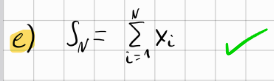
\includegraphics[width=0.8\linewidth]{images/lösungen/wts213e}\label{fig:figure40}
    \end{figure}
\end{auf}

\begin{auf}[(f) Begründen Sie, warum der Erwartungswert von $S_N$ existiert.]
    $\ $
    \begin{figure}[H]
        \centering
        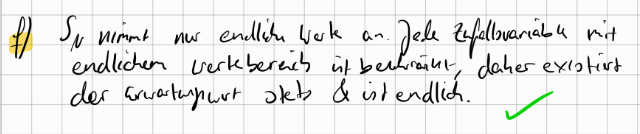
\includegraphics[width=0.8\linewidth]{images/lösungen/wts213f}\label{fig:figure39}
    \end{figure}
\end{auf}

\begin{auf}[(g) Berechnen Sie den Erwartungswert von $S_N$.]
    NOCH KEINE LÖSUNG % TODO NOCH KEINE LÖSUNG
\end{auf}